%% LaTeX-Beamer template for KIT design
%% by Erik Burger, Christian Hammer
%% title picture by Klaus Krogmann
%%
%% version 2.1
%%
%% mostly compatible to KIT corporate design v2.0
%% http://intranet.kit.edu/gestaltungsrichtlinien.php
%%
%% Problems, bugs and comments to
%% burger@kit.edu

\documentclass[18pt]{beamer}
\usepackage[utf8]{inputenc}
\usepackage{algpseudocode}
\usepackage{listings}
\usepackage{amsfonts} 
\usepackage{mathtools} 
%% SLIDE FORMAT

% use 'beamerthemekit' for standard 4:3 ratio
% for widescreen slides (16:9), use 'beamerthemekitwide'

\usepackage{templates/beamerthemekit}
% \usepackage{templates/beamerthemekitwide}

%% TITLE PICTURE

% if a custom picture is to be used on the title page, copy it into the 'logos'
% directory, in the line below, replace 'mypicture' with the 
% filename (without extension) and uncomment the following line
% (picture proportions: 63 : 20 for standard, 169 : 40 for wide
% *.eps format if you use latex+dvips+ps2pdf, 
% *.jpg/*.png/*.pdf if you use pdflatex)

%\TitleImage[width=\titleimagewd]{pics/title}
%\titleimage{}

%% TITLE LOGO

% for a custom logo on the front page, copy your file into the 'logos'
% directory, insert the filename in the line below and uncomment it

%\titlelogo{mylogo}

% (*.eps format if you use latex+dvips+ps2pdf,
% *.jpg/*.png/*.pdf if you use pdflatex)

%% TikZ INTEGRATION

% use these packages for PCM symbols and UML classes
% \usepackage{templates/tikzkit}
% \usepackage{templates/tikzuml}
\usepackage{listings}
\usepackage{color}

\definecolor{dkgreen}{rgb}{0,0.6,0}
\definecolor{gray}{rgb}{0.5,0.5,0.5}
\definecolor{mauve}{rgb}{0.58,0,0.82}

\lstset{frame=tb,
  language=Java,
  aboveskip=3mm,
  belowskip=3mm,
  showstringspaces=false,
  columns=flexible,
  basicstyle={\small\ttfamily},
  numbers=none,
  numberstyle=\tiny\color{gray},
  keywordstyle=\color{blue},
  commentstyle=\color{dkgreen},
  stringstyle=\color{mauve},
  breaklines=true,
  breakatwhitespace=true
  tabsize=3
}

% the presentation starts here

\title[Algo Tutorium Nr.1]{Algorithmen I - Sommersemester 2014}
\subtitle{Tutorium Nr. 1}
\author{Tobias Hornberger}

\institute{Institut für Theoretische Informatik}

\begin{document}

% change the following line to "ngerman" for German style date and logos
\selectlanguage{ngerman}

%title page
\begin{frame}
\titlepage
\end{frame}

%table of contents
%~ \begin{frame}[allowframebreaks]{Übersicht}
%~ \tableofcontents
%~ \end{frame}

\section{Einführung}
	\subsection{Vorstellung}
	\begin{frame}{Der Tutor}
		Tobias Hornberger
		\begin{itemize}
			\item 4. Semester Informatik
			\item Algorithmen I vor 2 Semestern gehört
			\item erstes Mal Tutor
		\end{itemize}
		Vorschläge/Anmerkungen/Feedback ist also sehr erwünscht
	\end{frame}

	\subsection{Kontakt}
	\begin{frame}{Kontakt}
		\begin{itemize}
			\item Email: \texttt{saibot1207@googlemail.com}
			\item Github: \texttt{https://github.com/Strandtasche}
			\item Bei Fragen per Email: Antwort an Alle
			Email mit Betreff "`Algo1Tut"' an mich schicken.
		\end{itemize}
	\end{frame}
	
	\begin{frame}{Namen}
		\centerline{\Huge{Vorstellungsrunde}}		
	\end{frame}

	\subsection{Organisatorisches}

	\begin{frame}{Organisation und Übungsbetrieb}
		\begin{itemize}
			\item Das Tutorium ist nicht dazu gedacht Übung/Vorlesung zu ersetzen, sondern als Ergänzung.
			\item Der Besuch wird empfohlen
			\item Keine Frontalveranstaltung
			\begin{itemize}
				\item Wenn Fragen auftauchen: einfach Fragen
				\item Es gibt keine dummen Fragen
			\end{itemize}
		\end{itemize}
	\end{frame}

	\begin{frame}{Organisation und Übungsbetrieb}
		Speziell für dieses Semester:
		\begin{itemize}
			\item Viele Feiertage fallen auf Donnerstage
			\item in diesen Wochen bitte andere Tutorien besuchen 
		\end{itemize}		
	\end{frame}

	\begin{frame}{Homepages}
		\begin{itemize}
			\item Vorlesungshomepage: \texttt{http://algo2.iti.kit.edu/AlgorithmenI2014.php}
			\begin{itemize}
				\item Interessante Organisatorische Details
				\item Vorlesungsfolien
				\item Die Übungsblätter
				\item Prof. Sanders Buch
				\item Literaturliste
			\end{itemize}
			\item Meine Folien: \texttt{https://github.com/Strandtasche/AlgoTutSS2014}
			\item ILIAS: \texttt{https://ilias.studium.kit.edu}
			\item Fakultät für Informatik $\rightarrow$ SS 2014 $\rightarrow$ Algorithmen I mit Übung			
		\end{itemize}		
	\end{frame}

	\begin{frame}{Übungsblätter}
		Das meiste wurde schon in der Vorlesung gesagt:
		\begin{itemize}
			\item 9 Tage Bearbeitungszeit: von Mittwoch bis Freitag der nächsten Woche
			\item Abgabe 12:45 Uhr im Kasten hier vor dem Raum (-118)
			\item 2er-Teams sind erlaubt
			\item Teamwechsel im Semester sind nicht vorgesehen, können aber in Sonderfälle mit Rücksprache durchgeführt werden
			\item Wichtig Wichtig: Tutoriumsnummer rechts oben groß auf die Abgabe!
			\item Kein Verpflichtender Übungsschein sondern Klausurbonus von 1/2/3 Punkten
			\item Zum ersten Mal dieses Jahr: Programmieraufgaben
			\begin{itemize}
				\item 4 Stück, über das Semester verteilt, in Java
				\item keine Klassenstrukturen sondern tatsächlich nur der Algorithmus
				\item Praktomat Abgabe: Ohne Verpflichtenden Code Style
				\item Dazu mehr wenn die erste Aufgabe kommt...
			\end{itemize}
		\end{itemize}		
	\end{frame}

\section{Pseudocode und Schleifeninvarianten}
	\subsection{Pseudocode}
	\begin{frame} {Pseudocode für FindMaximum} 
		Beispielcode:\\
		a ist ein Array von $\mathbb{N}$
		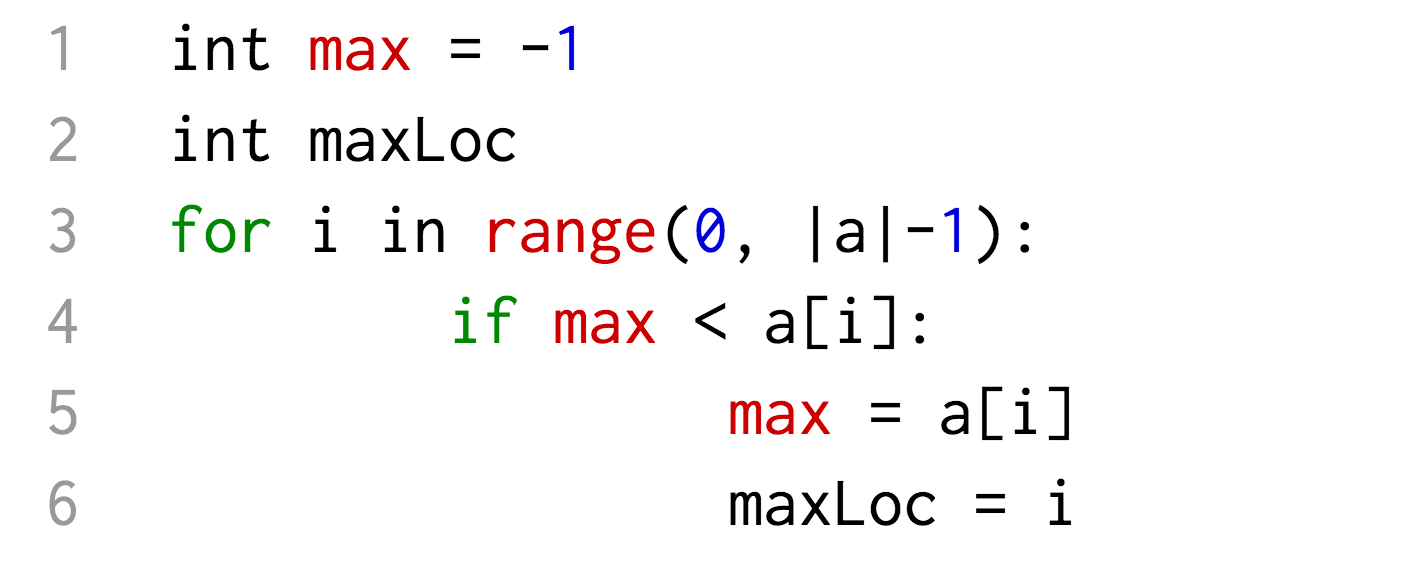
\includegraphics[align=center, scale=0.25]{pics/pseudocode01.png}		
	\end{frame} 

\section{Binary Search}
	\begin{frame}{Binäre Suche}
		Pseudocode: \\
		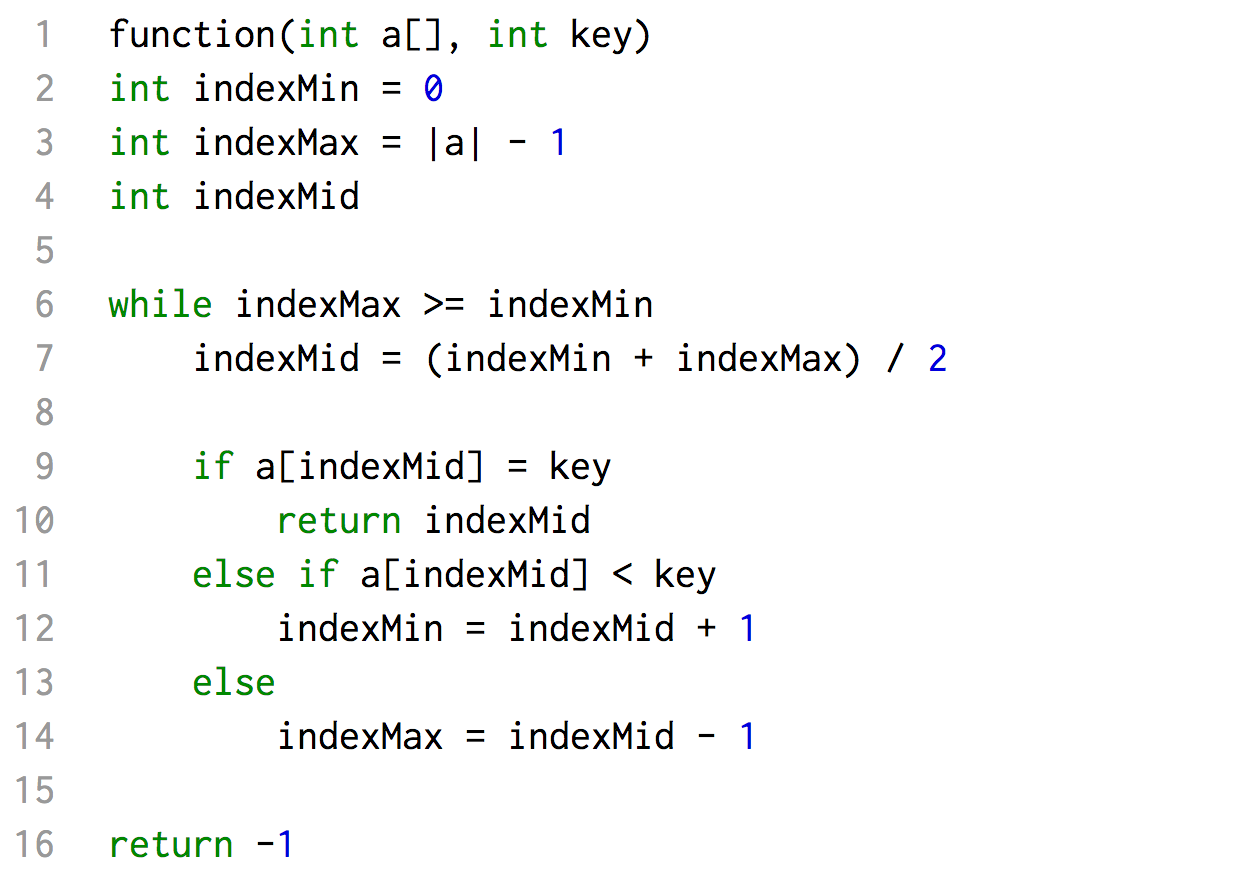
\includegraphics[align=center, scale=0.2]{pics/pseudocode03.png}			
	\end{frame}

\section{O-Kalkül}
	\subsection{Einführung}
	\begin{frame}{O-Kalkül}
		Bekannt aus GBI: \\
		zum Untersuchen von Laufzeitverhalten bei Eingaben verschiedener Größen
		\begin{itemize}
			\item \textbf{Best Case:} Cool zu wissen, aber meistens irrelevant
			\item \textbf{Average Case:} Sehr interessant, aber unhandlich/schwer zu berechnen
			\item \textbf{Worst Case:} Hiermit beschäftigen wir uns
		\end{itemize}
		\begin{block}{Bezug}
			Begriffe beziehen sich auf deterministische Algorithmen \\mit fester Eingabegröße.
		\end{block}
	\end{frame}

	\begin{frame}{Formale Definition}
				
		\begin{block} {Formeln}	
			\begin{itemize}
				\item{$\mathcal{O}(f(n)) = $ \{ g(n) : \exists c >  0 : \exists  n _{0} \in \mathbb{N} _{+} : \all n \geq n _{0} : g(n) \leq c * f(n) \}}

				\item{\Omega(f(n)) = \{ g(n) : \exists c >  0 : \exists  n _{0} \in \mathbb{N} _{+} : \all n \geq n _{0} : g(n) \leq c * f(n) \}}

				\item{\Theta(f(n)) = O(f(n))   \cap   \Omega(f(n))}
			
				\item{$o(f(n)) = $ \{ g(n) : \lim _{n \to \infty} \frac{g(n)}{f(n)} = 0 \}}

				\item{$\omega(f(n)) = $ \{ g(n) : \lim _{n \to \infty} \frac{g(n)}{f(n)} = \infty \}}

			\end{itemize}			
		\end{block}	

	\end{frame}

	\begin{frame}{Logarithmen mit verschiednen Basen}
		Bemerke: \\
		log(n) ist immer ohne Basis angegeben. Wieso?

		\begin{block} {Basisumrechnung}
			$ \log _{b} (n) = \frac{\log _{d} (n)}{\log _{d}(d)} $
		\end{block}

		\centerline{$\Rightarrow$ Ist das gleiche wie $ \frac{1}{\log _{d}(d)} * \log _{d} n $}
	\end{frame}

	\subsection{O-Kalkül Aufgaben}

	\begin{frame}{Aufgaben}
		\begin{itemize}
			\item $ 14 n ^{3} + 3 n ^{2}  + 7n + 15$
			\item $ 8 n + 7 $
			\item $ 15 n ^{2} + 3 $
			\item $ 1500 $
			\item $ -7 $
			\item $ n! $
			\item $ n ^{n} $
			\item $ \log{n} $
			\item $ \frac{1}{2} n ^{2} $
			\item $ n + n * \log{n} $
			\item $ 4 n + 15 n $	
		\end{itemize}	
	\end{frame}

	\begin{frame}{Beweisaufgabe}
		\begin{exampleblock}{Zeigen Sie, dass}
			\begin{itemize}
				\item $ \mathcal{O}( \log{n}) = \mathcal{O}( \log{n ^{2}} ) $
				\item $ f(n) =  n! $ \in $ \mathcal{O} ( n ^{n}) $ ist
			\end{itemize}
		\end{exampleblock}
	\end{frame}


	\begin{frame}{Bonusaufgabe}

		A ist ein Array aus $\mathbb{N}$, x ist ein int \\
		
\includegraphics[align=center, scale=0.25]{pics/pseudocode02.png}
		


		Was tut es? \\
		Laufzeit? \\
		Schleifeninvariante?	
	\end{frame}

	\begin{frame}{Bis zum nächsten Mal}
		
\includegraphics[align=center, scale=0.5]{pics/exploits_of_a_mom.png}
	\end{frame}

\end{document}
